\documentclass[tikz,border=10pt]{standalone}
\begin{document}
\begin{center}
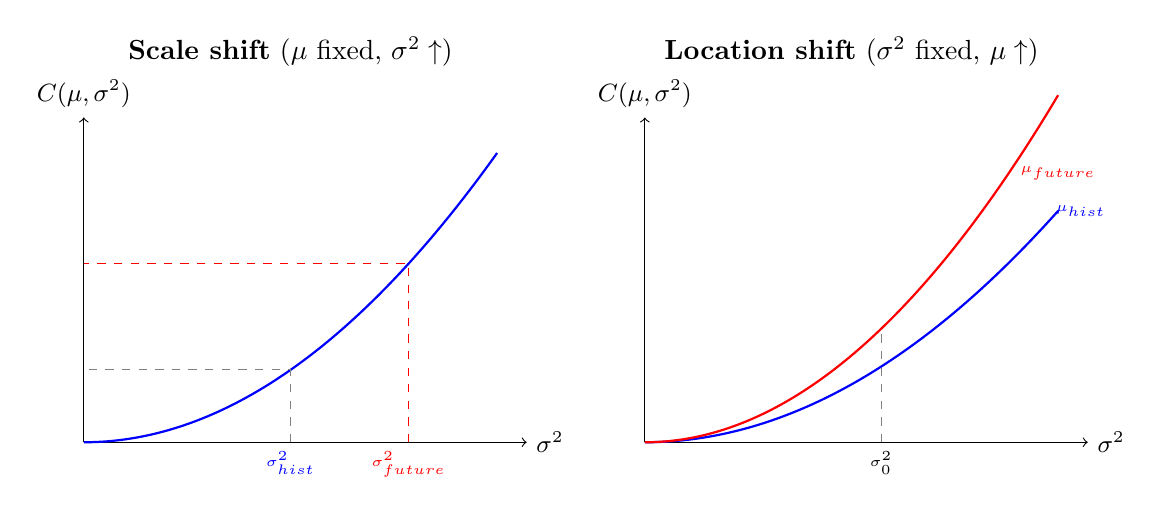
\begin{tikzpicture}[scale=0.75]
  % Left panel: scale shift
  \node[above] at (3.5, 6.2) {\textbf{Scale shift} ($\mu$ fixed, $\sigma^2 \uparrow$)};
  \draw[->] (0,0) -- (7.5,0) node[right] {\small $\sigma^2$};
  \draw[->] (0,0) -- (0,5.5) node[above] {\small $C(\mu,\sigma^2)$};
  \draw[thick, blue, domain=0:7, samples=100] plot (\x, {0.1*\x*\x});
  \draw[dashed, gray] (3.5,0) -- (3.5, {0.1*12.25}) -- (0, {0.1*12.25});
  \node[below, blue] at (3.5,0) {\tiny $\sigma^2_{hist}$};
  \draw[dashed, red] (5.5,0) -- (5.5, {0.1*30.25}) -- (0, {0.1*30.25});
  \node[below, red] at (5.5,0) {\tiny $\sigma^2_{future}$};
  % \draw[<->, thick, blue] (2.5, -0.35) -- (3.5, -0.35);
  % \node[below, blue] at (3.0, -0.35) {\tiny $\Delta\sigma^2$};
  % \draw[<->, thick, red] (4.5, -0.35) -- (5.5, -0.35);
  % \node[below, red] at (5.0, -0.35) {\tiny $\Delta\sigma^2$}; -->
  % Right panel: location shift
  \begin{scope}[xshift=9.5cm]
  \node[above] at (3.5, 6.2) {\textbf{Location shift} ($\sigma^2$ fixed, $\mu \uparrow$)};
  \draw[->] (0,0) -- (7.5,0) node[right] {\small $\sigma^2$};
  \draw[->] (0,0) -- (0,5.5) node[above] {\small $C(\mu,\sigma^2)$};
  % Lower curve (historical mu)
  \draw[thick, blue, domain=0:7, samples=100] plot (\x, {0.08*\x*\x});
  \node[right, blue] at (6.8, {0.08*49}) {\tiny $\mu_{hist}$};
  % Higher curve (future mu)
  \draw[thick, red, domain=0:7, samples=100] plot (\x, {0.12*\x*\x});
  \node[right, red] at (6.2, {0.12*38}) {\tiny $\mu_{future}$};
  % Same sigma^2 point
  \draw[dashed, gray] (4,0) -- (4, {0.12*16});
  \node[below] at (4,0) {\tiny $\sigma^2_0$};
  % Value brackets at same sigma^2
  % \draw[<->, thick, blue] (-0.3, {0.08*9}) -- (-0.3, {0.08*16});
  % \node[left, blue] at (-0.3, {0.08*12.5}) {\tiny $V|_{\mu_h}$};
  % \draw[<->, thick, red] (-0.8, {0.12*9}) -- (-0.8, {0.12*16});
  % \node[left, red] at (-0.8, {0.12*12.5}) {\tiny $V|_{\mu_f}$}; -->
  \end{scope}
\end{tikzpicture}
\end{center}
\end{document}